\documentclass[]{report}
\usepackage{graphicx, float}
\usepackage[export]{adjustbox}

\title{\centering CSP334 : Computer Networks \\Lab Assignment No 1\\Assignment on Wireshark}
\author{\LARGE Sahil\\2016UCS0008}

% to use proper section numbering in the report type 
\renewcommand{\thesection}{\arabic{section}}

\begin{document}

\maketitle

%%%%%%%%%%%%%%%%%%%%%%%%%%%%%%%%%%%%%%%%%%%%%%%%
\section{Network Interface:}
The network interfaces available on the computer are shown in the snapshot below. They include \textbf{Wi-Fi}, virtual wireless interface \textbf{p2p0}, Thunderbolt bridge, Thunderbolt 1, Software Network interface (gif0) and tunnel interface (stf0).
\begin{figure}[H]
	\vspace{0pt}
	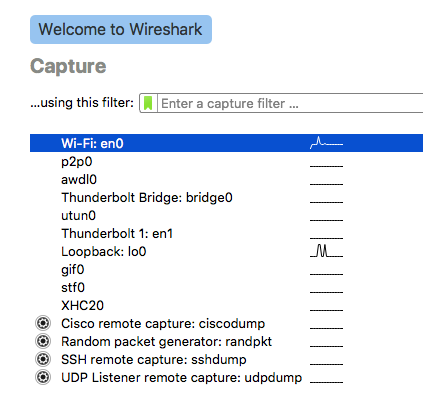
\includegraphics[height = 350pt, keepaspectratio]{Snapshots/q1.png}
\end{figure}
\textbf{Wi-Fi} network interface was eventually selected.

%%%%%%%%%%%%%%%%%%%%%%%%%%%%%%%%%%%%%%%%%%%%%%%%
\section{Application Layer protocol used:}

\begin{figure}[H]
	\vspace{0pt}
	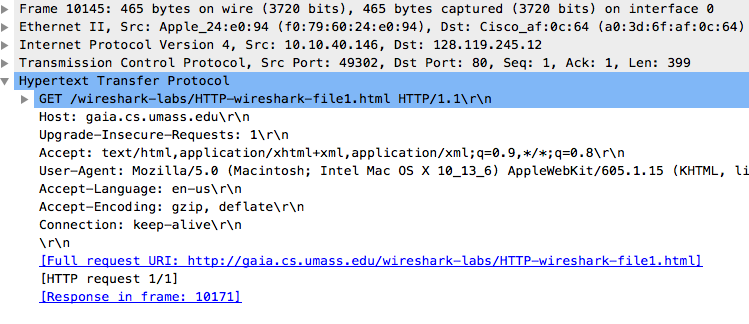
\includegraphics[height = 175pt, keepaspectratio]{Snapshots/q2.png}
\end{figure}

The application layer protocol used is \textbf{HTTP}, i.e. HyperText Transfer Protocol, as highlighted in the frame captured.
%%%%%%%%%%%%%%%%%%%%%%%%%%%%%%%%%%%%%%%%%%%%%%%%
\section{Other protocols used:}

\begin{figure}[H]
	\vspace{0pt}
	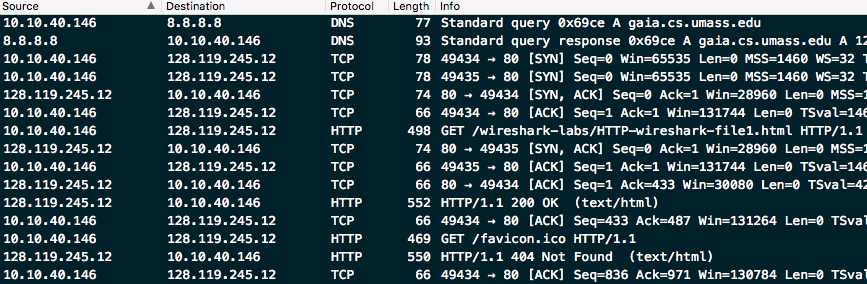
\includegraphics[height = 133pt, keepaspectratio]{Snapshots/q3.png}
\end{figure}

The other protocols used are \textbf{DNS} which in turn used UDP and \textbf{TCP}. 
\\
 \textbf{IP} is not displayed in the packet listing window since it is always used. 
%%%%%%%%%%%%%%%%%%%%%%%%%%%%%%%%%%%%%%%%%%%%%%%%
\section{IPA of source and destination:}

\begin{figure}[H]
	\vspace{0pt}
	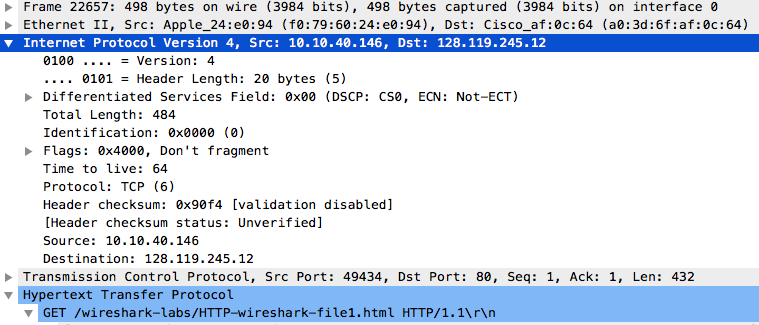
\includegraphics[height = 175pt, keepaspectratio]{Snapshots/q4_1.png}
\end{figure}

The IPA of the \textbf{source machine} is: $10.10.40.146$ 
\\
The IPA of the \textbf{destination machine} is: $128.119.245.12$
\\ \\
We can ascertain that the IPA of the destination is indeed the same as that observed in the wireshark by either entering the IPA in the web browser since its an HTTP request, or we can do ping to the web address requested to get its IPA. \\
Another alternative way is to look at the following \textbf{DNS} packet captured, which clearly mentions the resolved IPA of the requested website, which is the destination.
\begin{figure}[H]
	\vspace{0pt}
	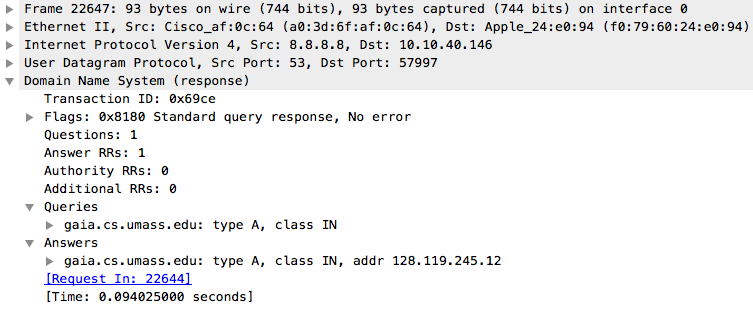
\includegraphics[height = 175pt, keepaspectratio]{Snapshots/q4_2.png}
\end{figure}

%%%%%%%%%%%%%%%%%%%%%%%%%%%%%%%%%%%%%%%%%%%%%%%%
\section{Class of IPA:}


%%%%%%%%%%%%%%%%%%%%%%%%%%%%%%%%%%%%%%%%%%%%%%%%
\section{Frame: Information about packet}
The no. of bits captured in the HTTP packet: $3984$ 
\\
The time at which the packet was captured: Sep 10, 2018 $08:24:17.473788000$ IST
\begin{figure}[H]
	\vspace{0pt}
	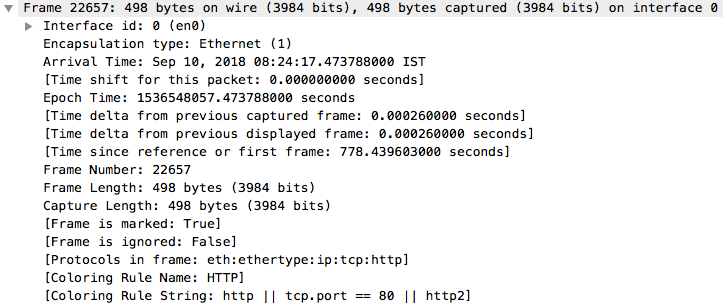
\includegraphics[height = 175pt, keepaspectratio]{Snapshots/q6.png}
\end{figure}

%%%%%%%%%%%%%%%%%%%%%%%%%%%%%%%%%%%%%%%%%%%%%%%%
\section{Interface ID and address of interface:}
The interface ID used is: $0$ (en0)
\\
The address of the interface is: f0:79:60:24:e0:94.
\begin{figure}[H]
	\vspace{0pt}
	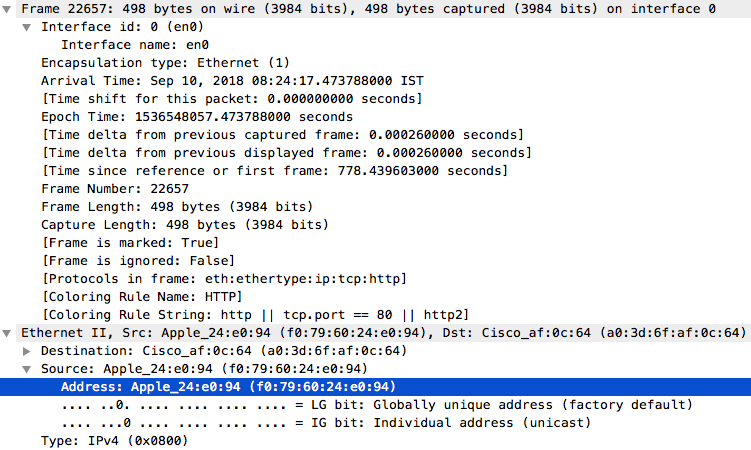
\includegraphics[height = 200pt, keepaspectratio]{Snapshots/q7.png}
\end{figure}

%%%%%%%%%%%%%%%%%%%%%%%%%%%%%%%%%%%%%%%%%%%%%%%%
\section{Time taken between HTTP GET and HTTP OK reply:}
The HTTP GET message sent and the HTTP OK reply are highlighted, the time taken = $17.768101 - 17.473788$ = $0.294313$ seconds.
\begin{figure}[H]
	\vspace{0pt}
	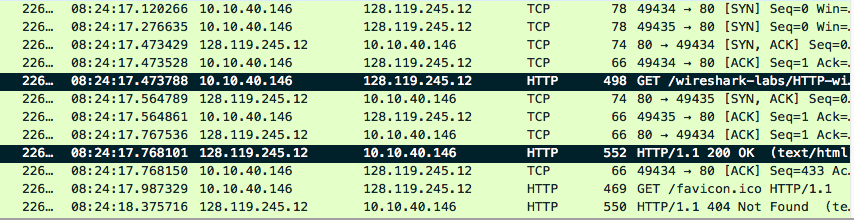
\includegraphics[height = 105pt, keepaspectratio]{Snapshots/q8.png}
\end{figure}

%%%%%%%%%%%%%%%%%%%%%%%%%%%%%%%%%%%%%%%%%%%%%%%%
\section{HTTP GET and OK messages:}
The HTTP GET and OK messages are as shown below:
\begin{figure}[H]
	\vspace{0pt}
	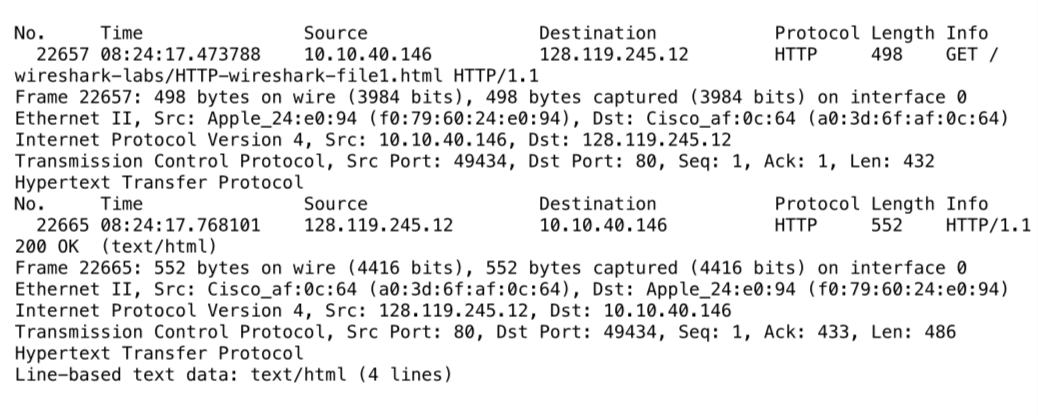
\includegraphics[height = 135pt, keepaspectratio]{Snapshots/q10.png}
\end{figure}

%%%%%%%%%%%%%%%%%%%%%%%%%%%%%%%%%%%%%%%%%%%%%%%%
\section{Destination physical address of the first packet captured and device it belongs to:}
\begin{figure}[H]
	\vspace{0pt}
	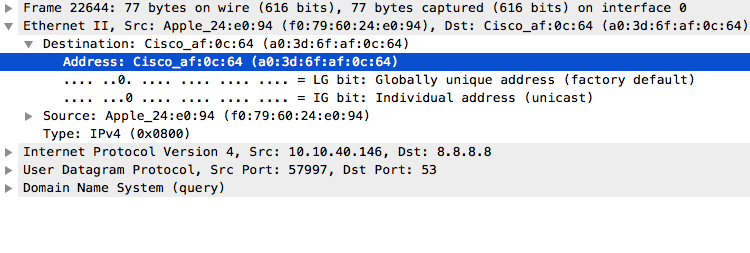
\includegraphics[height = 135pt, keepaspectratio]{Snapshots/q11.png}
\end{figure}
The destination physical address of the first packet (HTTP) captured is \textbf{a0:3d:6f:af:0c:64} and it belongs to the device Cisco.

%%%%%%%%%%%%%%%%%%%%%%%%%%%%%%%%%%%%%%%%%%%%%%%%
\section{Bytes of header in the first frame:}


%%%%%%%%%%%%%%%%%%%%%%%%%%%%%%%%%%%%%%%%%%%%%%%%
\section{How to know if Ethernet header contains an IP packet?}

\begin{figure}[H]
	\vspace{0pt}
	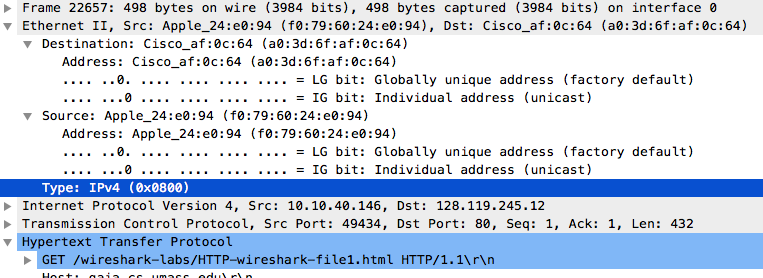
\includegraphics[height = 145pt, keepaspectratio]{Snapshots/q13.png}
\end{figure}
We can determine by looking at the Ethernet header of the frame whether it contains an IP packet since the field \textbf{Type} contains this detail as highlighted above. 

%%%%%%%%%%%%%%%%%%%%%%%%%%%%%%%%%%%%%%%%%%%%%%%%
\section{How to know if the first packet captured has TCP or UDP as transport protocol by looking at the IP header?}
We can know whether the packet captured has TCP or UDP as transport protocol by looking at the \textbf{Protocol} field in the IP header. If we consider DNS as the first packet captured, it has UDP whereas considering HTTP as the first packet, it has TCP. 
\begin{figure}[H]
	\vspace{0pt}
	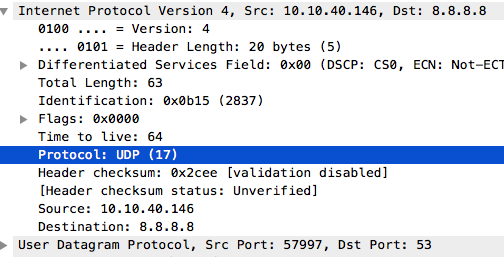
\includegraphics[height = 135pt, keepaspectratio]{Snapshots/q14.png}
\end{figure}

%%%%%%%%%%%%%%%%%%%%%%%%%%%%%%%%%%%%%%%%%%%%%%%%
\section{Source and destination ports in the SYN, ACK:}

\begin{figure}[H]
	\vspace{0pt}
	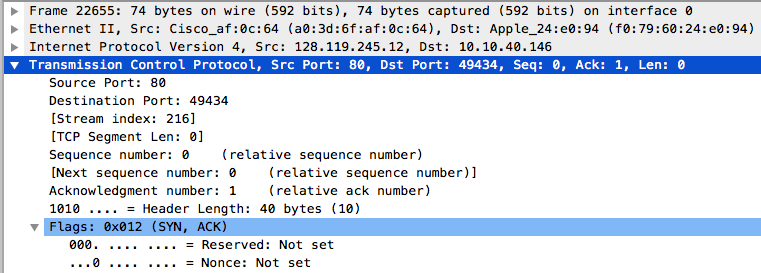
\includegraphics[height = 145pt, keepaspectratio]{Snapshots/q15.png}
\end{figure}

%%%%%%%%%%%%%%%%%%%%%%%%%%%%%%%%%%%%%%%%%%%%%%%%
\section{Server Hello message has 1 as relative sequence number and 185 as relative acknowledgement number:}

\begin{figure}[H]
	\vspace{0pt}
	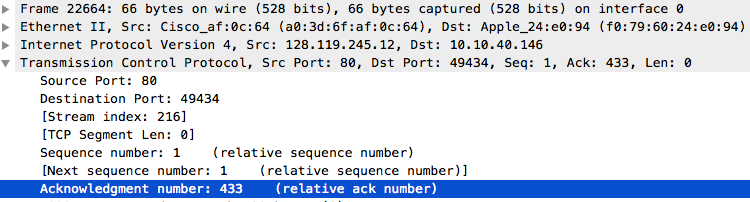
\includegraphics[height = 105pt, keepaspectratio]{Snapshots/q16.png}
\end{figure}

%%%%%%%%%%%%%%%%%%%%%%%%%%%%%%%%%%%%%%%%%%%%%%%%
\section{First sequence number sent by the server to the client:}

\begin{figure}[H]
	\vspace{0pt}
	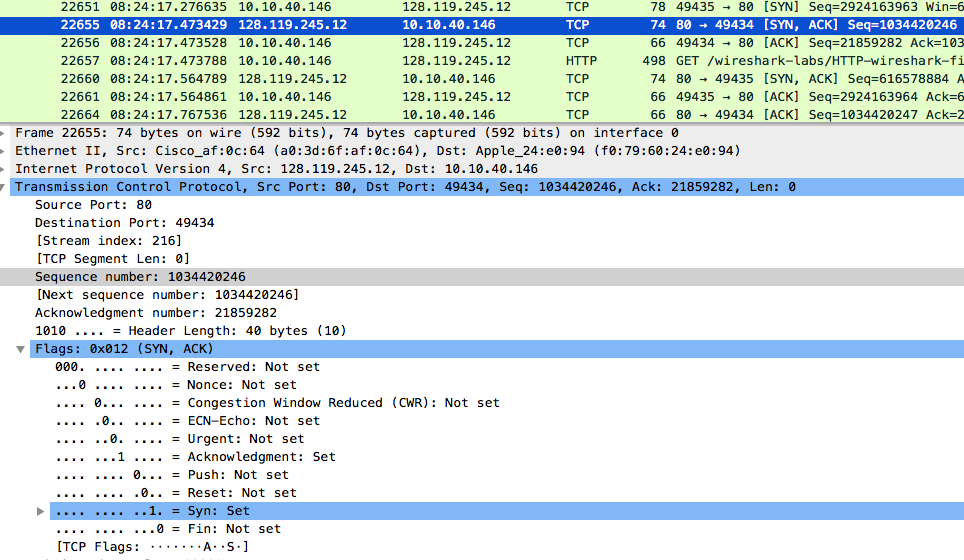
\includegraphics[height = 230pt, keepaspectratio]{Snapshots/q17.png}
\end{figure}

\end{document}